\section{Felhasználói dokumentáció}
Ez a fejezet tartalmazza a segítséget egy sikerese regisztráció illetve bejelentkezés használatához. A felhasználói műveletek alapvetően két csoportra bonthatóak:
\begin{itemize}
\item Azok a műveletek amiket a felhasználó a telefonjána böngészőjében hajt végre
\item És a telefonra telepített bejelentkezést segítő android alkalmazás kezelése
\end{itemize}

Egy sikeres bejelentkezéshez ennek megfelelően futnia kell egy weboldalnak amely előre definiált módon csatlakozik az E-Group IDX felhasználó-hitelesítési és azonosítási termékéhez.
A szakdolgozat keretein belül egy AngularJS weboldalt JavaEE (Spring keretrendszer) backend réteggel hoztunk létre és integráltuk a bejelentkezést a Spring Security rendszerébe.

\subsection{Mobil eszköz minimum követelményei}
A rendszer működése többnyire egy LG G3 telefonnal volt tesztelve, gyors és megbízható eredmények így a következő követelmények teljesülése esetén garantálhatóak.
\begin{itemize}
\item Minimum SDK 21-es verzió (Lollipop), Android 5.0
\item Minimum 2GB RAM
\item Quad-core 2.5 GHz Krait 400 CPU vagy erősebb
\item Előlapi kamera
\end{itemize}

Természetesen ennél gyengébb eszközökön is fut az alkalmazás amennyiben minimum a 16-os SDK szintet (Jelly Bean) elére, és rendelkezik előlapi kamerával, ám a teljesítmény drasztikusan csökkenhet, szélsőséges esetben a bejelentkezéshez szükséges képtranszformációk sem kerülnek végrahajtásra, így a folyamat megszakadhat és a kérés elutasításra kerülhet.

\subsection{Mobil alkalmazás telepítése}
A mobil alkalmazás telepítését a telpítendő apk fájl birtokában azt megnyitva lehet elkezdeni. A műveletsor elején az android rendszer hozzáférést kér képkészítéshez, és NFC kommunikációhoz, ezek nélkül a telepítés nem tud folytatódni mivel elengedethetetlenek az alkalmazás megfelelő működéséhez (13. ábra).
\\Miután minden komponens települt azt egy sikeres telepítést jelző felirat jelzi (14. ábra).
\begin{figure}[h]
 \begin{minipage}{.5\textwidth} 
\centering
    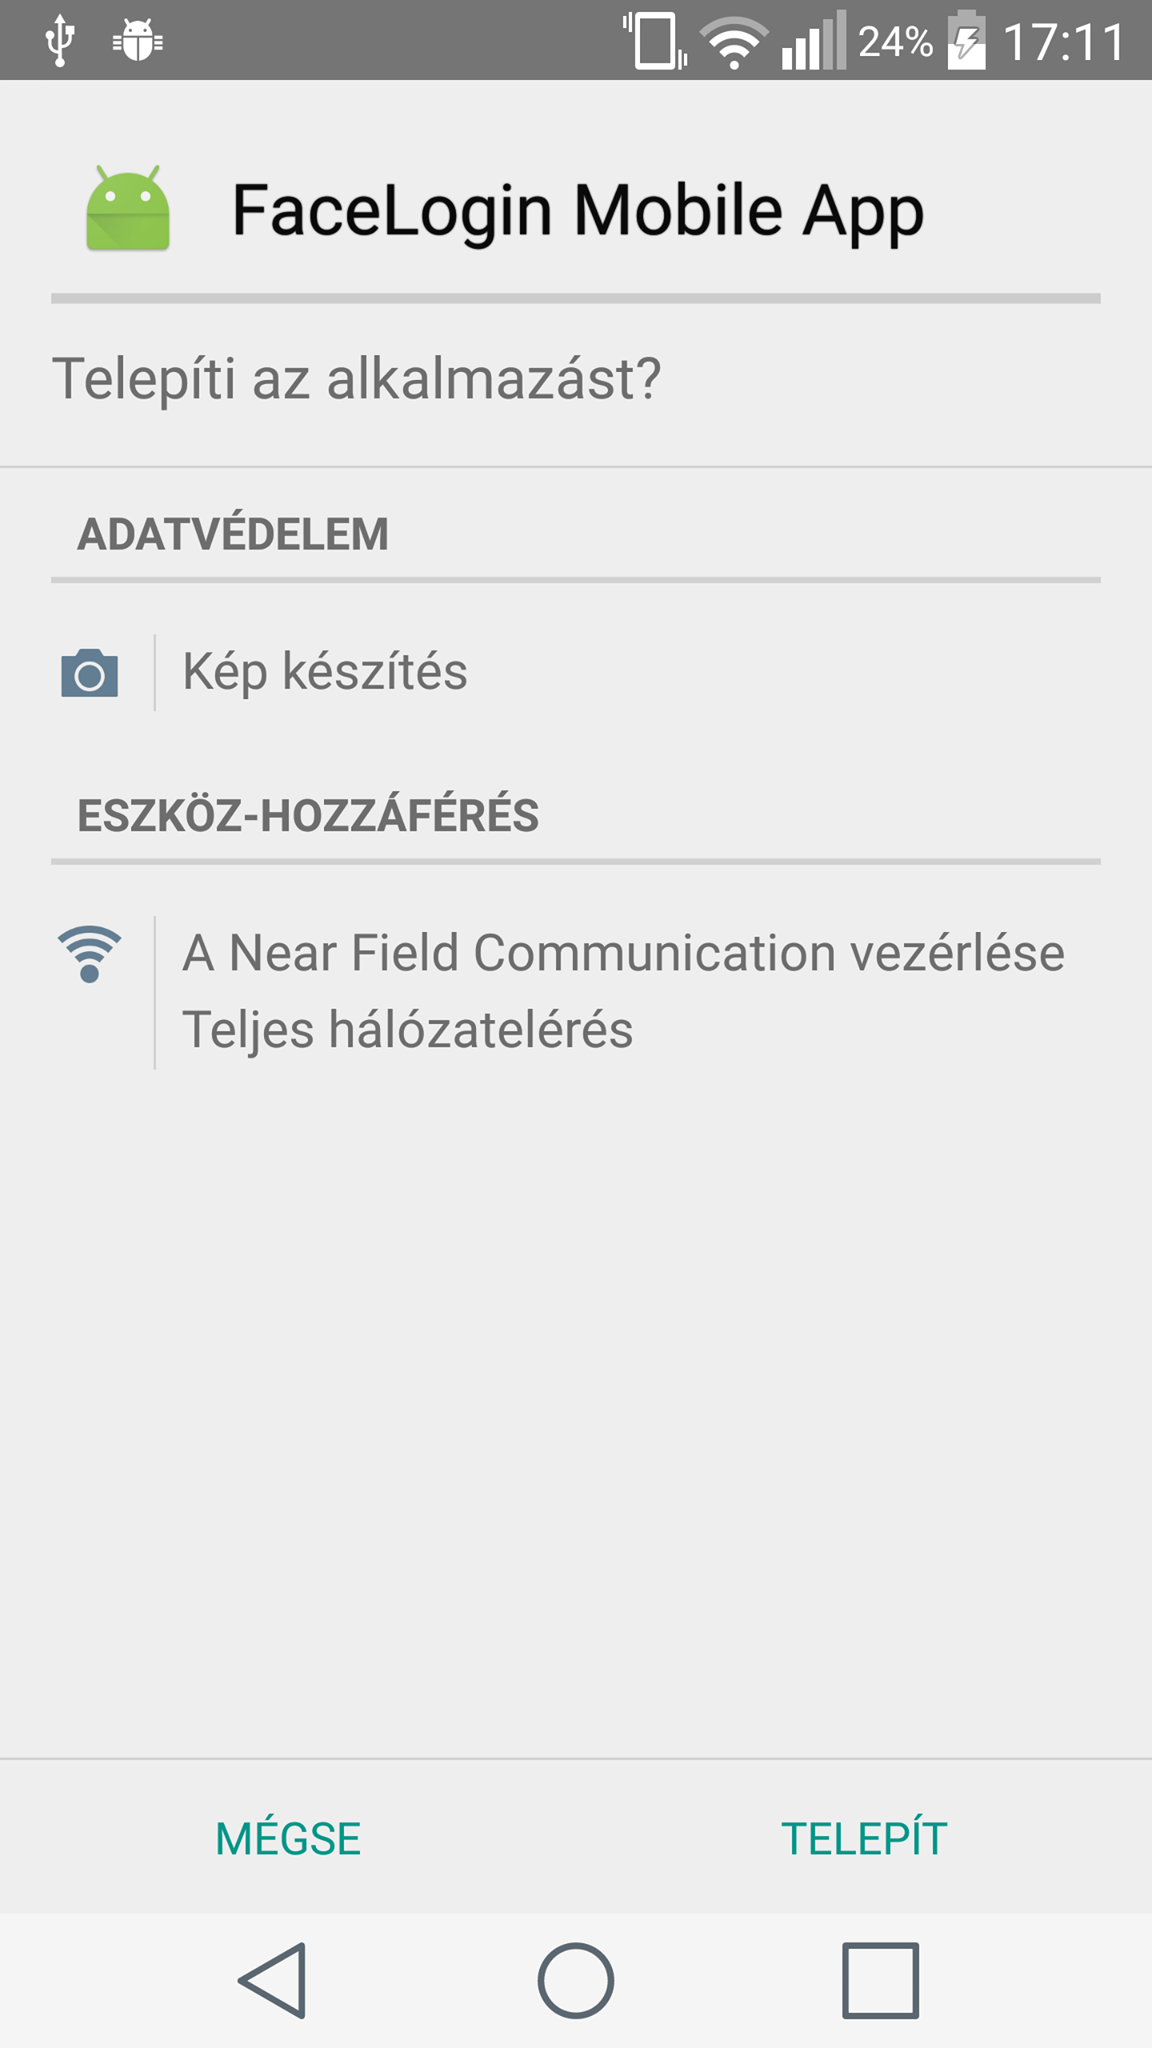
\includegraphics[scale=0.10]{img/install_app}
    \caption{Hozzáférések kérése}
 \end{minipage}
 \begin{minipage}{.5\textwidth} 
\centering
     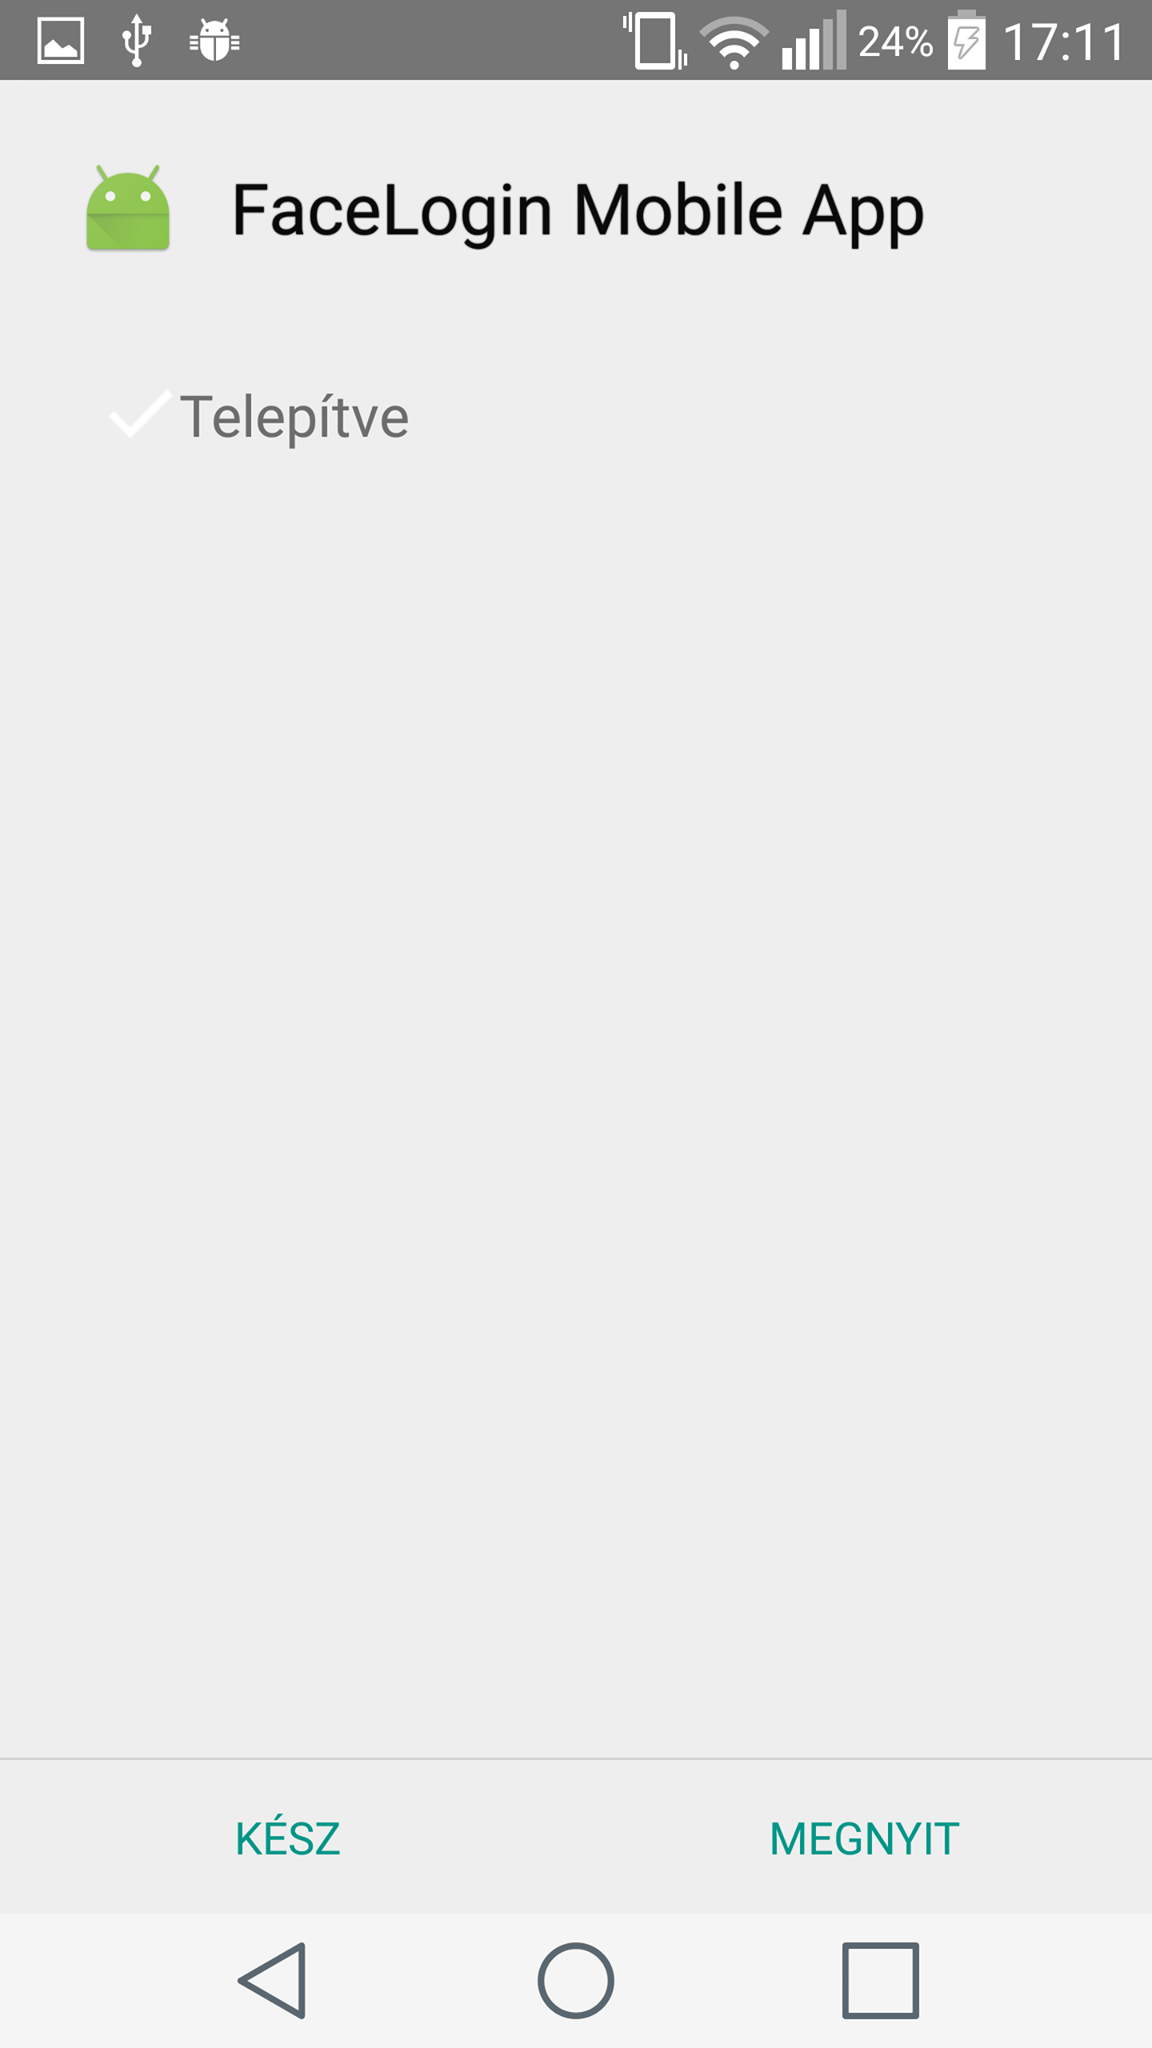
\includegraphics[scale=0.10]{img/app_installed}
     \caption{Telepítés sikeres}
 \end{minipage}
\end{figure}

\subsection{A webalkalmazás követelményei}
Az egyetlen követelmény hogy csatlakozzon  E-Group IDX felhasználó-hitelesítési és azonosítási termékének egy olyan verziójához amiben megtalálható már a szakdolgozat keretében elkészített modul. Az integrálás módjáról a fejlesztői dokumentációban lehet olvasni.

\subsection{Az authentikáló alkalmazás követleményei}

Ez a modul egy Wildfly 10.1.0 verziójú szerveren fut, Java 8-as verzió alatt. Az indítási paraméterek között szerepel a
\begin{verbatim}
-Xms64m -Xmx512m 
\end{verbatim}
bejegyzés amely a minimum illetve a maximum allokálandó memóriát szabja meg. Ekkora memóriaterületen a rendszer működése megbízható, így ez minimum követelménynek tekinthető.

\subsection{A regisztráció folyamata}
A regisztráció folyamatát a rendszer működéséhez készített demonstrációs weboldalon keresztül mutatom be. Fontos megjegyezni, hogy akármilyen honlapra a weboldal technológiájától függően gyorsan vagy nehezebben, de integrálható a bejelentkezési modul, amennyiben az IDX szerveren be van állítva hogy fogadja a kéréseket az adott címről.
\\A folyamat végrehajtásához az egész műveletsor Android mobiltelefonról kell hogy végrehajtódjon, személyi számítógépről az alkalmazás nem fog megnyílni, és így nem lehetséges bejelentkezni!
\\Az oldal megnyitását követően a publikus főoldal látható. A regisztrációs oldalra való jutáshoz a Sign Up feliratra kell kattintani a bejelentkezés doboz alatt (1.kép). A linkre kattintva megjelenik a regisztrációs felület (2. kép). A szövegmezőbe kattintva adhatjuk meg a felhasználónevünket, majd a "START REGISTRATION" gombra kattintva indíthatjuk a regisztrációs folyamatot. Hibalehetőségek, amik esetén a műveletet megszakítja a rendszer és lehetőséget ad új felhazsnálónév megadására:
\begin{itemize}
\item A megadott felhasználónév már létezik a rendszerben (3. kép)
\item Nincsen megadva felhasználónév (4.kép)
\end{itemize}

Amennyiben a megadott név szabad, úgy egy új gomb jelenik meg "OPEN APP" felirattal (5.kép). 
Erre a gombra kattintva a már feltelepített alkalmazás megnyílik, és a további információkat szolgáltatja.

\newpage